\documentclass[12pt, a4paper,oneside]{article}

\usepackage{graphicx}
\graphicspath{ {references/} }

\usepackage{todonotes}

\usepackage{float}%figures placed HERE

\usepackage[backend=bibtex]{biblatex}
\bibliography{miniproject}
%\bibliographystyle{plain}


\title{Reconfigurable and Low Energy Systems Miniproject\\\large CORDIC}
\author{Anders Normann Poulsen (apouls16@student.aau.dk)\\Gabriel Vasluianu (gvaslu16@student.aau.dk)}


\begin{document}

\maketitle
\newpage
\section{Introduction}
CORDIC is an algorithm that computes trigonometric functions (and many other)
by using simple operations.
%https://en.wikipedia.org/wiki/CORDIC
A typical application would be a two-dimensional vector rotation, as seen in 
figure \ref{fig:two_vector}. Here $(x_{in}, y_{in})$ are the initial coordinates
of the vector, and $(x_{out}, y_{out})$ are the final coordinates.

\begin{figure}[h]
	\centering
	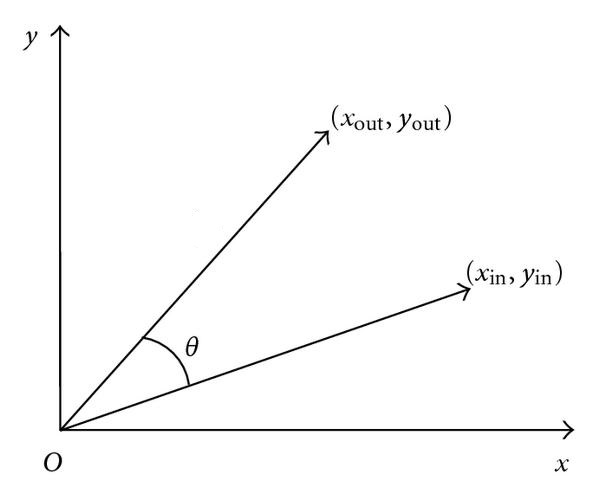
\includegraphics[width = 7cm]{two_vector.jpg}
	\caption{Two dimensional vector rotation}
	\label{fig:two_vector}
\end{figure}

In order to achieve the operation of rotating the vector, the following equations
have to be calculated:
\[ x_{out} = x_{in} cos\theta - y_{in} sin\theta \]
\[ y_{out} = x_{in} sin\theta + y_{in} cos\theta \]

As seen here, the hardware computing these equations would have to do:
four multiplications, two addition/subtraction 
and access a lookup table for the trigonometric functions\cite{cordic1}.
Keep in mind that multiplication is an expensive operation, and a multiplicator
takes a large area. This is the reason why we want to use CORDIC in some 
applications.
\\

The idea CORDIC introduces is that we can compute the new coordinates by 
iterating through an algorithm that constantly tries to get closer to the 
final result, using a table containing angles to be used in the next iteration
(micro-rotation). These angles can be either added or subtracted in order
to take the next step, and approximate the target, as seen in figure \ref{fig:cordic_iterations}.

\begin{figure}[h]
	\centering
	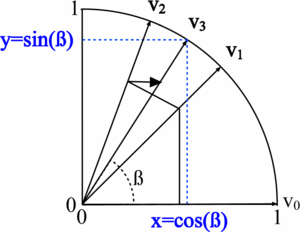
\includegraphics[width = 7cm]{cordic_iterations.png}
	\caption{Ilustration of cordic iterations}
	\label{fig:cordic_iterations}
\end{figure}

\todo[inline]{redo the figure}
The generalized equations of the CORDIC algorithm are:
\[ x_{i+1} = x_i - \sigma_i \cdot 2^{-i} \cdot y_i \]
\[ y_{i+1} = y_i - \sigma_i \cdot 2^{-i} \cdot x_i \]
\[ z_{i+1} = z_i - \sigma_i \cdot arctan(2^{-i}) \]

%https://en.wikibooks.org/wiki/Trigonometry/For_Enthusiasts/The_CORDIC_Algorithm

Here, $x_{i+1}$ and $y_{i+1}$ show us the values respective to each iteration.
In order to know what to do in the next iteration (add/subtract from the previous
angle), we need to compute $\sigma_i$. This is done by looking at the value of 
$z_i$:

$$
\sigma_i = \left\{ \begin{array}{rl}
 +1 &\mbox{ if $z_i>=0$} \\
 -1 &\mbox{ if $z_i<0$}
       \end{array} \right.
$$

$z_i$ keeps track of how much we rotated at every iteration and subtracting that 
from the wanted angle.
The values of $x_i$ and $y_i$ need to be scaled by a factor of $K_i$:

$$K_i = \frac{1}{\sqrt{1 + 2^{-2i}}}$$

However, there are several methods to do this by calculating it in advance or by 
making it a constant. For small architectures, this aspect can be disregarded.
\\
These being said, by looking at the equations we can see that we will need 
to apply the following operations: addition, bitshift and comparison.

\section{The algorithm}


\begin{figure}[H]
	\centering
	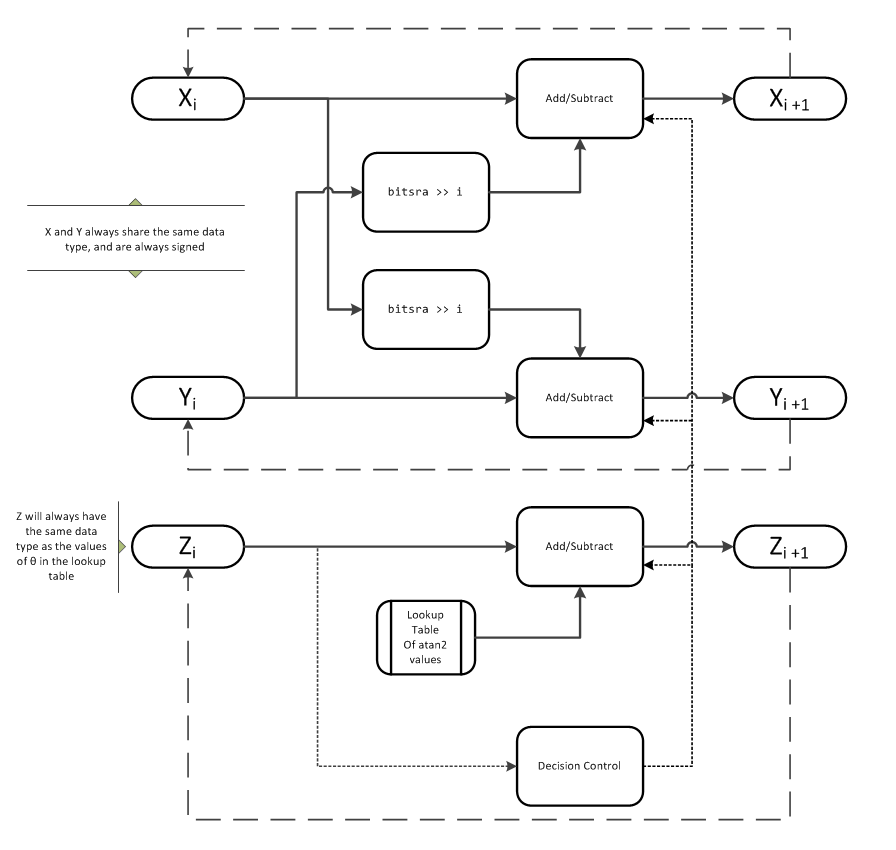
\includegraphics[width = \linewidth]{cordic_rotationkernel.png}
	\caption{The CORDIC algorithm}
	\label{fig:cordic_algorithm}
\end{figure}

\printbibliography

\end{document}